\documentclass[12pt]{beamer}

% Choose how your presentation looks.
%
% For more themes, color themes and font themes, see:
% http://deic.uab.es/~iblanes/beamer_gallery/index_by_theme.html
%
\mode<presentation>
{

  \usetheme{Boadilla}      % or try Darmstadt, Madrid, Warsaw, ...
  \usecolortheme{seahorse} % or try albatross, beaver, crane, ...
  %\usefonttheme{structurebold}
  %\usefonttheme{serif}
  \usefonttheme{professionalfonts}  % or try serif, structurebold, professionalfonts ...
  \setbeamertemplate{navigation symbols}{} % hide the navigation symbols
  \setbeamertemplate{caption}[numbered]
  
} 

\setbeamertemplate{blocks}[rounded][shadow=true]% 要将上述示例幻灯片中围绕定理的盒子改成圆角并添加阴影
%\usepackage{ctex} % Chinese
\usepackage[english]{babel}
\usepackage[utf8x]{inputenc}
\usepackage{color}
\usepackage[orientation=landscape,size=custom,width=16,height=9,scale=0.5,debug]{beamerposter}%修改比例,16:9
\usepackage{sidecap}
\usepackage{graphicx}

\def\mathfamilydefault{\rmdefault}

%\usepackage[colorlinks,linkcolor=blue,anchorcolor=blue,citecolor=green,CJKbookmarks=True]{hyperref}
\logo{
\includegraphics[width=3cm]{figs/f1.png}}% add logo
\setbeamercovered{dynamic}  % translucent when using pause
\useinnertheme{rectangles}
\renewcommand{\theequation}{\arabic{section}-\arabic{equation}}% 设置公式编号格式
\renewcommand{\thefigure}{\arabic{section}-\arabic{figure}} % 设置图像编号格式
\newtheorem{procedure}{Procedure}




%%%%%%%%%%%%%%%%%%%%%%%%%%%%%%%%%%%%%%%%%%% the inforamtion of coverpage
\title[]{Comparison of Spectral Estimation Methods for Current Estimation by an HF Surface Wave Radar}
\author[HU S.K.]{HU, Senkang}
\institute[BIT]{School of Information and Electronics\\ 
Beijing Institute of Technology\\
Beijing, China, 100081\\[1ex]
{\color{blue} \textit{\href{mailto:1120183150@bit.edu.cn}{1120183150@bit.edu.cn}}}\\

}

\date{May, 2021}
%%%%%%%%%%%%%%%%%%%%%%%%%%%%%%%%%%%%%%%%%%%

%\linespread{1.1}

\begin{document}

\begin{frame}
  \titlepage
\end{frame}


% Uncomment these lines for an automatically generated outline.
\begin{frame}{Outline}
  \tableofcontents
\end{frame}

\section{Introduction}
\begin{frame}{Outline}
  \transfade%淡入淡出效果
  \tableofcontents[sectionstyle=show/shaded,subsectionstyle=show/shaded] %这几个参数我也不知道该如何准确地解释,反正它们最终的效果是突出显示当前章节,而其它章节都进行了淡化处理
  %\addtocounter{framenumber}{-1}  %目录页不计算页码
\end{frame}


\begin{frame}{1. Introduction}
  \begin{itemize}
    \item {\color{magenta} Conventional spectrum estimation method}, such as the periodogram method
    \item {\color{magenta} Modern techniques}, such as the autoregressive method and multiple signal classification methods
    
  \end{itemize}
\end{frame}
\begin{frame}{1. Introduction}
  \begin{itemize}
    \item For calculate the radial current velocity, it is important to estimate its associate Doppler shift from { the frequency spectrum.}\pause
    \item In addition to the conventional centroid method, a more robust Bragg frequency identification method, termed the {\color{magenta} symmetric-peak-sum}, is proposed and examined in conjunction with each of the spectral estimation techniques. 
  \end{itemize}
\end{frame}
\begin{frame}{1. Introduction}
  \begin{itemize}
    \item It has been found that a weighted sum of the radar-derived current estimates using these two methods generally provides a lower rms difference from the buoy measurements. 
    \item The weighting ratio is optimized using a genetic algorithm
    \item Field data indicate that a combination of these spectral estimation methods is capable of providing improvements in retrives current velocities for various current conditions.
  \end{itemize}
\end{frame}

\begin{frame}{1. Introduction}{High frequency surface wave radar (HFSWR)}
  \begin{itemize}
    \item High frequency surface wave radar (HFSWR) systems are a cost-effective tool for remote sea-state sensing and are well known for current mapping.
    \item High frequency surface wave radar takes advantage of the short wave (3$\sim$30MHz) diffracted propagation and low attenuation on the conductive ocean surface, and uses the vertically polarized antenna to radiate the radio waves. It can detect the moving targets such as ships, aircraft, icebergs and missiles that appear below the line of sight on the sea level {\color{magenta} beyond the horizon}, and the action range can reach more than 300km.
  \end{itemize}
\end{frame}

\begin{frame} 
  \begin{figure}
    \centering
    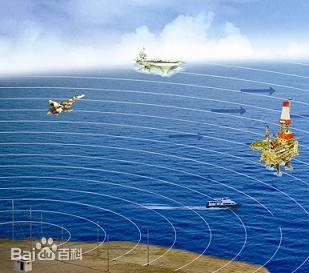
\includegraphics[width=0.5\linewidth]{figs/f5.jpg}
    \caption{Schematic diagram of application of high frequency surface wave radar (HFSWR)}
  \end{figure}
\end{frame}
\begin{frame} 
  \begin{figure}
    \centering
    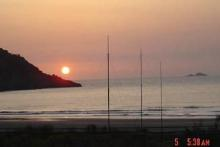
\includegraphics[width=0.7\linewidth]{figs/f6.jpg}
    \caption{The medium range high frequency surface wave radar system developed by Wuhan University}
  \end{figure}
\end{frame}


\begin{frame}{1. Introduction}{High frequency surface wave radar (HFSWR)}
  \begin{itemize}
    \item At the same time, using the first-order scattering and second-order scattering mechanism of the sea surface to the high frequency electromagnetic wave, the high frequency ground wave radar can extract sea state information such as wind field, wave field and current field from the radar echo, so as to realize the real-time monitoring of the Marine environment in a large range, with high precision and all weather.
    \item It is widely used in military field and Marine environment detection field
  \end{itemize}
\end{frame}


\begin{frame}{1. Introduction}{High frequency surface wave radar (HFSWR)}
  \begin{itemize}
    \item High frequency surface wave radar (HFSWR) systems are a cost-effective tool for remote sea-state sensing and are well known for current mapping.
    \item The power spectrum of the received signal, which for these coherent radars is a Doppler spectrum, typicallly consist of two large peaks which arise from Bragg resonant scattering of the signal from ocean gravity waves of halfs the radio wavelength.
    \item This so-called Bragg peaks occur at positive and negetive Doppler for waves moving towards or away from the radar.
  \end{itemize}
\end{frame}
\begin{frame}
  \begin{figure}[htbp]
    \centering
    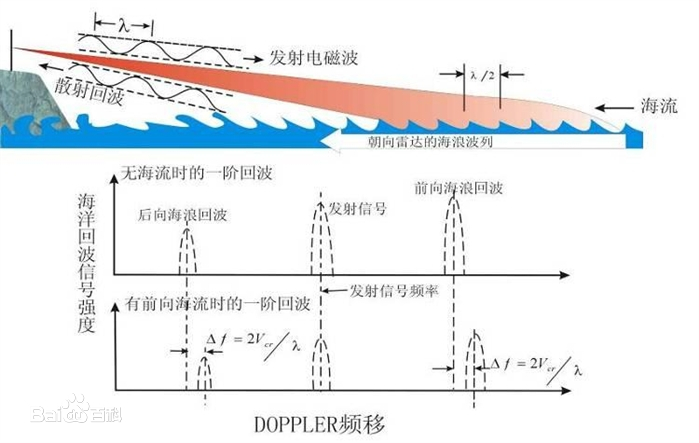
\includegraphics[width=0.7\linewidth]{figs/f7.jpg}
    \caption{Shore-based ground wave radar detection principle diagram}
  \end{figure}  
\end{frame}

\begin{frame}{1. Introduction}{High frequency surface wave radar (HFSWR)}
  \begin{itemize}
    \item The associated Bragg frequency shift in the backscatter signal is used to determine surface currents. 
    \item For still water and an operating frequency of $f$, due to the speed of the Bragg waves, the Bragg peaks appear at Doppler frequencies given by\begin{equation}
      f_b=\pm \sqrt{\frac{gf}{\pi c}}
    \end{equation}
    where $c$ and $g$ are the speed of the light and the acceleration due to gravity.
  \end{itemize}
\end{frame}
\begin{frame}{1. Introduction}{High frequency surface wave radar (HFSWR)}
  \begin{itemize}
    \item When a uniform surface current exists, both peaks will be shifted in the same direction by an amount of \begin{equation}
      \Delta f_c=\frac{2v_c f}{c}
    \end{equation}
    where $v_c$ is the radial component of the surface surrent along the radar look direction.\pause
    \item The most important radar parameter for
    current mapping is {\color{magenta} the resolution of the Doppler spectrum estimation (SE)} and {\color{magenta} the resulting accurate     identification of the Bragg frequency}
  \end{itemize}
\end{frame}

\begin{frame}{1. Introduction}
  But there are two main difficulties in estimating $\Delta f_c$ :
  \begin{enumerate}
    \item There are various SE methods from which to choose
    \item Difficulty asises in estimating the Bragg shift directly based on the identification of the maximum amplitude.
  \end{enumerate}\pause
  Broadening of the Bragg peaks, which may arise from current fluctuations or contamination by ionospheric clutter, can be very significant under certain sea states. Even in ideal conditions, an inherent randomness associated with the spectral amplitudes is observed, and this also translates into a fluctuation in the Bragg peak locations.
\end{frame}


\section{Spectrum Estimation Methods}
\subsection{Welch Method}
\begin{frame}{Outline}
  \transfade%淡入淡出效果
  \tableofcontents[sectionstyle=show/shaded,subsectionstyle=show/shaded] %这几个参数我也不知道该如何准确地解释,反正它们最终的效果是突出显示当前章节,而其它章节都进行了淡化处理
  %\addtocounter{framenumber}{-1}  %目录页不计算页码
\end{frame}
\begin{frame}{2.1. Welch Method}


  {\large The standerd periodogram method:}\newline

The periodogram of an $L$-point sequence, $x(0), x(1),\cdots, x(L-1)$, is defined as
\begin{equation}
  S\left(f_{k}\right)=\frac{1}{L}\left|\sum_{n=0}^{L-1} x(n) e^{-j 2 \pi n f_{k} T}\right|
\end{equation}

Where $T$ is the sampling rate.
  
\end{frame}

\begin{frame}{2.1. Welch Method}

  In order to reduce the noise caused by {\color{red} imperfect and finite data}, \pause so the Welch Method is introduced in exchange for reducing the frequency resolution.
  
\end{frame}
\begin{frame}{2.1. Welch Method}{The Procedure of Welch Method}
  \begin{procedure}
   \begin{enumerate}
    \item The sequence $x(n)$ is divided into $K$ segments of length $M$, overlappd by $P$ percent.\pause
    \item Each segment is multiplied by a window function prior to computing the periodogram.\pause
    \item Then, the power spectral estimate is obtained by averaging the periodograms for the $K$ segments.
  \end{enumerate} 
  \end{procedure}
  
   
\end{frame}

\begin{frame}{2.1. Welch Method}{The advantage of Welch Method}
  The advantage of the Welech method over the standerd periodofram method is that the {\color{red} variance can be reduced} by overlapping and averaging.
  
\end{frame}

\begin{frame}{2.1. Welch Method}{An Example of the advantage}
  \begin{example}
    When $K$ segments are averaged, the variance of the average, $\sigma^2_{ave}$, is related to the individual variance of the segments, $\sigma^2_{ind}$, for a special case of 75\% overlap as:
  \begin{equation}
    \frac{\sigma_{{ave }}^{2}}{\sigma_{{ind }}^{2}}=\frac{1}{K}\left\{1+2 \operatorname{cor}^{2}(0.75)+2 \operatorname{cor}^{2}(0.5)\right\}
  \end{equation} 
  Where $\operatorname{cor}(P)$ is the correlation existing between successive window transforms having a overlap of $P$ percent\cite{TRETHEWEY2000267}.
  \end{example}
\end{frame}

\begin{frame}{2.1. Welch Method}{An Example of the advantage}
  \begin{example}
     \begin{itemize}
    \item It is clear that the variance in the Welch Method as compared to the periodogram method is {\color{red} reduced by a factor $K$}.
    \item The Welch method has been commonly used in HF radar spectral estimation, but the {\color{red} frequency resolution} of the required FFT limits the precise of the current estimate.
  \end{itemize}
  \end{example}
 
   
\end{frame}


\subsection{Autoregressive (AR) Method}
\begin{frame}{Outline}
  \transfade%淡入淡出效果
  \tableofcontents[sectionstyle=show/shaded,subsectionstyle=show/shaded] %这几个参数我也不知道该如何准确地解释,反正它们最终的效果是突出显示当前章节,而其它章节都进行了淡化处理
  %\addtocounter{framenumber}{-1}  %目录页不计算页码
\end{frame}
\begin{frame}{2.2. Autoregressive (AR) Method}{Brief introduction of AR method}
  \begin{itemize}
    \item In statistics, econometrics and signal processing, an autoregressive (AR) model is a representation of a type of random process; as such, it is used to describe certain time-varying processes in nature, economics, etc.
    \item The autoregressive model specifies that the output variable depends linearly on its own previous values and on a stochastic term (an imperfectly predictable term);
  \end{itemize}
      
\end{frame}
\begin{frame}{2.2. Autoregressive (AR) Method}{Brief introduction of AR method}
  \begin{itemize}
    \item thus the model is in the form of a stochastic difference equation (or recurrence relation which should not be confused with differential equation).
    \item Together with the moving-average (MA) model, it is a special case and key component of the more general autoregressive–moving-average (ARMA) and autoregressive integrated moving average (ARIMA) models of time series, which have a more complicated stochastic structure;
    
  \end{itemize}
\end{frame}
\begin{frame}{2.2. Autoregressive (AR) Method}{Brief introduction of AR method}
  \begin{itemize}
    \item it is also a special case of the vector autoregressive model (VAR), which consists of a system of more than one interlocking stochastic difference equation in more than one evolving random variable.
    \item Contrary to the moving-average (MA) model, the autoregressive model is not always stationary as it may contain a unit root.
  \end{itemize}
\end{frame}
\begin{frame}{2.2. Autoregressive (AR) Method}
  As one of the two main categories of high-resolation SE mathod, AR is a model-based method, the parameters of which are estimated from a given data sequence $X_t,0\leq t\leq N-1$. \pause
  The data can be modeled as output of casual, all-pole, discrete filter whose input is white noise, given by
  \begin{equation}
    X_{t}=c+\sum_{i=1}^{p} \varphi_{i} X_{t-i}+\varepsilon_{t}
  \end{equation}
  where $\varphi_{1}, \ldots, \varphi_{p}$ are the parameters of the model, $c$ is a constant, and $\varepsilon_t$ is white noise.
\end{frame}



\begin{frame}{2.2. AR Method}{Definition}
   This can be equivalently written using the backshift operator $B$ as
  \begin{equation}
    X_{t}=c+\sum_{i=1}^{p} \varphi_{i}B^i X_{t}+\varepsilon_{t}
  \end{equation}\pause
  so that, moving the summation term to the left side and using polynomial notation, we have\begin{equation}
    \phi[B] X_{t}=c+\varepsilon_{t}
  \end{equation}
  An autoregressive model can thus be viewed as the output of an all-pole infinite impulse response filter whose input is white noise.
\end{frame}


\begin{frame}{2.2. AR Method}{Definition}
  Some parameter constraints are necessary for the model to remain wide-sense stationary.\pause
  \begin{example}
    Process in the $AR(1)$ model with $|\varphi_1|\geq 1$ are not stationary. More generally, for an $AR(p)$ model to be wide-sense stationary, the roots of the polynomial $\Phi(z):=1-\sum_{i=1}^{p} \varphi_{i} z^{p-i}$ must lie outside the unit circle.
  \end{example}
\end{frame}

\begin{frame}{2.2. AR Method}
  The power spectral density (PSD) estimate is then computed from $\varphi_i$ and $\sigma^2$\cite{abc}, as given by 
  \begin{equation}
    P_{A R}(f)=\frac{T {\color{red} \sigma^{2}}}{\left|1+\sum_{k=1}^{p} {\color{red} \varphi_i} e^{-j 2 \pi k f T}\right|^{2}}
  \end{equation}
\end{frame}
\subsection{MUSIC}
\begin{frame}{Outline}
  \transfade%淡入淡出效果
  \tableofcontents[sectionstyle=show/shaded,subsectionstyle=show/shaded] %这几个参数我也不知道该如何准确地解释,反正它们最终的效果是突出显示当前章节,而其它章节都进行了淡化处理
  %\addtocounter{framenumber}{-1}  %目录页不计算页码
\end{frame}
\begin{frame}{2.3. MUSIC}
  Another main category of the high-resolution SE
methods is the {\color{magenta} subspace method}, of which MUSIC
is a commonly-used example. It generates frequency component estimates for signal based on an Eigen-analysis of the autocorrelation matrix.The MUSIC frequency estimater, which is based on noise subspace eigenvectors $U_N$ and a vector $a(\theta)$ of complex sinusoidal components, is given by \begin{equation}
  P_{ {MUSIC }}=\frac{1}{a^{H}(\theta) \hat{U}_{N} \hat{U}_{N}^{H} a(\theta)}
\end{equation}
  where $H$ represents tht conjugate transpose.
\end{frame}

\begin{frame}{2.3. MUSIC}
  The DOA mathematical model of the narrow band far field signal is
  \begin{equation}
    X(t)=A(\theta)s(t)+N(t)
  \end{equation}
  The covariance matrix of the array matrix is
  \begin{equation}
    R=E\left[X X^{H}\right]=A E\left[S S^{H}\right] A^{H}+\sigma^{2} I=A R_{S} A^{H}+\sigma^{2} I
  \end{equation}
\end{frame}
\begin{frame}{2.3. MUSIC}
  Since the signal and noise are independent of each other, the data covariance matrix can be decomposed into signal and noise,$AR_SA^H$ is the part of signal.

  We do the eigendecomposition of R,\begin{equation}
    R=U_SV_SU_S^H+U_NV_NU_N^H
  \end{equation}
  The first term of the formula {\color{magenta} $U_S$ is the signal subspace }spanned by large eigenvalues corresponding to eigenvectors, and the second term {\color{magenta} $U_N$ is the noise subspace} spanned by small eigenvalues corresponding to eigenvectors.
\end{frame}
\begin{frame}{2.3. MUSIC}
  Since the signal and noise are independent under ideal conditions, the signal subspace and noise subspace are orthogonal to each other, and the guide vector in the signal subspace is orthogonal to the noise subspace
  \begin{equation}
    a^H(\theta)U_N=0
  \end{equation}\pause
  Based on this property, classical MUSIC algorithm can be obtained. Considering that the actual received data matrix is of finite length, the maximum likelihood estimate of the data covariance matrix is\begin{equation}
    \hat{R}=\frac{1}{L} \sum_{i=1}^{L} X X^{H}
  \end{equation}
\end{frame}
\begin{frame}{2.3. MUSIC}
  The eigenvector matrix $\hat{U}_N$ of noise subspace can be calculated by eigendecomposition of $\hat{R}$. Due to the existence of noise, A and UN are not completely orthogonal, so DOA is realized by the minimum optimization search,\begin{equation}
    \theta_{M U S I C}=\operatorname{argmin}a^{H}(\theta) \hat{U}_{N} \hat{U}_{N}^{H} a(\theta)
  \end{equation}\pause
  Therefore, the spectrum estimation formula of MUSIC algorithm is\begin{equation}
    P_{ {MUSIC }}=\frac{1}{a^{H}(\theta) \hat{U}_{N} \hat{U}_{N}^{H} a(\theta)}
  \end{equation}
  
\end{frame}
\begin{frame}{2.3. MUSIC}
  An example of the MUSIC estimated spectrum using the same field data as in Fig.\ref{f2} is show in Fig.\ref{f3}.
  \begin{figure}[htbp]
    \centering
    \caption{Power spectral density estimation by AR}
    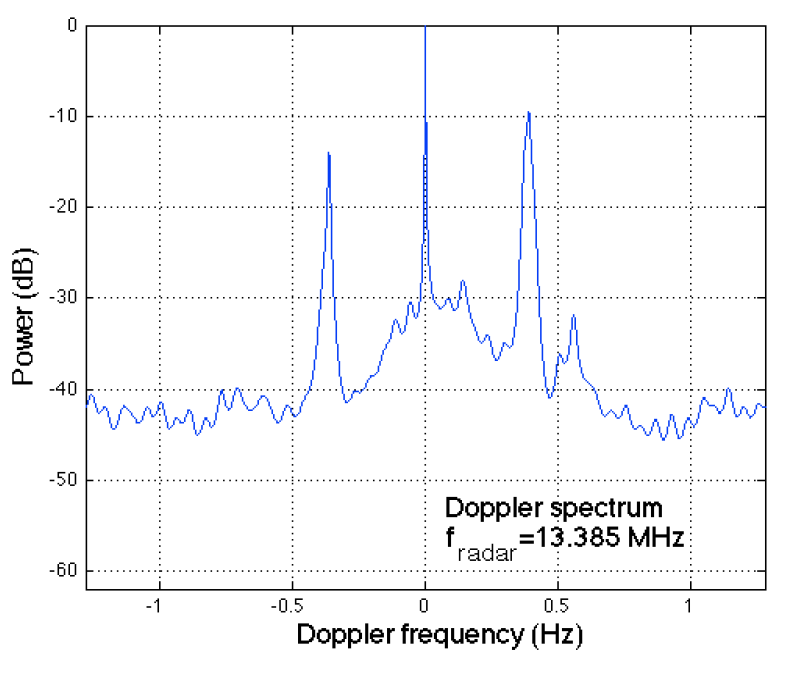
\includegraphics[width=0.4\linewidth]{./figs/f2.png}
    \label{f2}
  \end{figure}
\end{frame}

\begin{frame}{2.3. MUSIC}
  An example of the MUSIC estimated spectrum using the same field data as in Fig.\ref{f2} is show in Fig.\ref{f3}.
  \begin{figure}[htbp]
    \centering
    \caption{Power spectrum density estimation by MUSIC}
    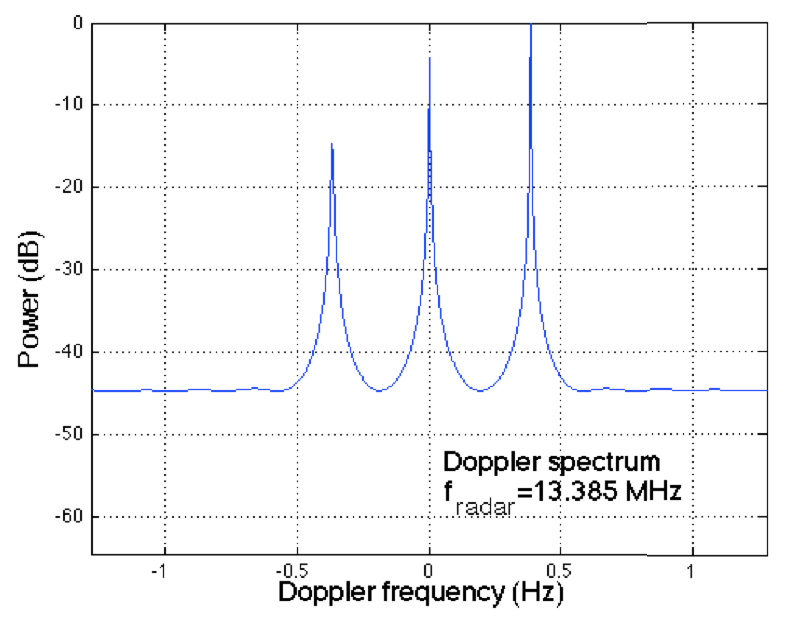
\includegraphics[width=0.4\linewidth]{./figs/f3.png}
    \label{f3}
  \end{figure}
\end{frame}

\begin{frame}{2.3. MUSIC}
  \begin{itemize}
    \item It is clearly seen that, compared  with the AR method, the MUSIC algorithm is able to provide frequency estimates with higher resolulation.
    \item The MUSIC method is sentive to  the conditioning of the autocorrelation matrix.
    \item Under low SNR conditions, if signal subspace is small, the autocorrelation matrix may be ill-conditioned and the MUSIC algorithm may fenerate false spectral peaks.
  \end{itemize}
   
\end{frame}


\section{Bragg Peak Frequency Identification}
\begin{frame}{Outline}
  \transfade%淡入淡出效果
  \tableofcontents[sectionstyle=show/shaded,subsectionstyle=show/shaded] %这几个参数我也不知道该如何准确地解释,反正它们最终的效果是突出显示当前章节,而其它章节都进行了淡化处理
  %\addtocounter{framenumber}{-1}  %目录页不计算页码
\end{frame}

\begin{frame}{3. Bragg Peak Frequency Identification}{Brief Introduction}\begin{itemize}
  \item In HF radar data, the Bragg Doplpler exhibits time-varying and width-broadening features. 
  \item The amplitude of the Rayleigh random process, is due to the random phases of the waves on the scattering surface. The Bragg peak is also spread in frequency. 
  \item No matter which waveforms are used (pulses or FM modulated waveforms), the transmitted signal is spread over a bandwidth and will cause a certain degree of Bragg broadening determained by the pulse width or sweep bandwidth.
\end{itemize}
\end{frame}

\begin{frame}{3. Bragg Peak Frequency Identification}{Brief Introduction}\begin{itemize}
  \item  Also, an increase of the half-power beamwidth of the receiving antenna from 0.5 to 4 degree will broaden the Bragg frequency by 30\%. 
  \item Considering the time-varying and width-broadening features discussed above, two Bragg Doppler shift identification methods are proposed.
\end{itemize}
\end{frame}

\subsection{Centroid Method}
\begin{frame}{Outline}
  \transfade%淡入淡出效果
  \tableofcontents[sectionstyle=show/shaded,subsectionstyle=show/shaded] %这几个参数我也不知道该如何准确地解释,反正它们最终的效果是突出显示当前章节,而其它章节都进行了淡化处理
  %\addtocounter{framenumber}{-1}  %目录页不计算页码
\end{frame}
\begin{frame}{3.1. Centroid Method}
  The commonly used 'centroid' method is considered
here to estimate the {\color{red} mean or center frequency}
of the Bragg peak having narrow but finite width. \pause
\begin{procedure}
  \begin{enumerate}
  \item In this method, a small Doppler region determined
by the largest expected current speed in the radar
experiment area and centered on the Bragg peak
having the higher signal-to-noise ratio (SNR), is
isolated first.
    \item The centroid frequency for this region
of the Doppler spectrum is calculated by weighting
the frequency components with the SNR values in
the region. The SNR values at each frequency used
in the weighting should be above 10 dB.
\end{enumerate}
\end{procedure}
\end{frame}

\subsection{Symmetric-peak-sum (SPS)}
\begin{frame}{Outline}
  \transfade%淡入淡出效果
  \tableofcontents[sectionstyle=show/shaded,subsectionstyle=show/shaded] %这几个参数我也不知道该如何准确地解释,反正它们最终的效果是突出显示当前章节,而其它章节都进行了淡化处理
  %\addtocounter{framenumber}{-1}  %目录页不计算页码
\end{frame}
\begin{frame}{3.2. Symmetric-peak-sum (SPS)}
  The presence of swell or target peaks will affect the SNR values at those frequencies and may thus negatively influence the centroid calculation. To reduce the impact of swell and targets, the SPS method is proposed.  \pause
  \begin{procedure}
    \begin{enumerate}
      \item Two spectral regions centered on $+f_b$ and $-f_b$ are first identified. 
      \item Then, these regions are superposed completely and averaged.
      \item A maximum in the averaged signal is considered to be the power at the Bragg frequency.
    \end{enumerate}
  \end{procedure}
\end{frame}

\subsection{Optimal Weighting}
\begin{frame}{Outline}
  \transfade%淡入淡出效果
  \tableofcontents[sectionstyle=show/shaded,subsectionstyle=show/shaded] %这几个参数我也不知道该如何准确地解释,反正它们最终的效果是突出显示当前章节,而其它章节都进行了淡化处理
  %\addtocounter{framenumber}{-1}  %目录页不计算页码
\end{frame}
\begin{frame}{3.3. Optimal Weighting}
  It is found that a weighted sum of the current estimates using the centroid method ($v_{c1}$) and the SPS method ($v_{c2}$) generally provides lower root mean square (RMS) differences from the buoy measurments than using each of these alone. The weighting process is given by\begin{equation}
    v_c(t)=(1-r)*v_{c1}(t)+r*v_{c2}(t)
  \end{equation}
  where $r$ is the weighting ratio. 
\end{frame}
\begin{frame}{3.3. Optimal Weighting}
  An optimization problem of the weighting ratio is first attempted using the Nelder-Mead method, which is a gradient search method known for \begin{itemize}\pause
    \item being vulnerable to being {\color{magenta} trapped on local extrema}
    \item possible {\color{magenta} low convergence near the extrema}
  \end{itemize}\pause
   In this case, another approach, termed the genetic algorithm (GA), is considered.
\end{frame}

\begin{frame}{3.3. Optimal Weighting}{Genetic Algorithm (GA)}
  In the GA algorithm , a population of candidate solutions to an optimization problem is evolved toword a better solution. The definition of the problem is made in terms of the 
  \begin{enumerate}
    \item parameters space ($R$)
    \item the objective space ($Y$)
    \item an objective function ($\mu$)
  \end{enumerate}
  Initially, candidate solutions are randomly selected.
\end{frame}

\begin{frame}{3.3. Optimal Weighting}
  \begin{itemize}
    \item   During each iteration in the evolution, they are altered or mutated. According to its fitness to the problem, some are retained for the next iteration while others are discarded.
    \item Fitness here refers to the value of the objective function in the optimization problem.
    \item The algorithm terminates when either a maximum number of iterations has been produced, or a satisfactory fitness level has been reached. 
    \item Seeking the optimal ratio of the current estimates using the two Bragg identification methods is fomulated into a single parameter and single objective problem. 
  \end{itemize}
\end{frame}
\begin{frame}{3.3. Optimal Weighting}
   To find the weighting ratio $r$ belonging to the peremater space $r\in R$, $y$ is minimized in the objective space $Y$ through the objective function mapping $\mu$: $R\rightarrow Y$ as
   \begin{equation}
     \{r_{opt}\}=\min_{r\in R}(\mu(r))
   \end{equation}
   
   The rms difference between the buoy and the weighted radar current measurements is calculated in the objective function and is considered the figure of merit. The lower the difference, the better fit will be. For the Welch, AR, and the MUSIC method, the opotimal ratio $r$ is found to be 85\%, 75\%, and 100\%, respectively.
\end{frame}


\section{Ground-Truth Data Validation}
\begin{frame}{Outline}
  \transfade%淡入淡出效果
  \tableofcontents[sectionstyle=show/shaded,subsectionstyle=show/shaded] %最终的效果是突出显示当前章节,而其它章节都进行了淡化处理
  %\addtocounter{framenumber}{-1}  %目录页不计算页码
\end{frame}

\begin{frame}{4. Ground-Truth Data Validation}
    The methods discussed above were evaluated
    using {\color{magenta} HF radar data} collected from Nov. 29th, 2012
    to Aug. 21st, 2013 at Placentia Bay, Newfoundland
    in conjunction with with the deployment of two
    oceanographic buoys
\end{frame}

\begin{frame}
  \begin{figure}[htbp]
      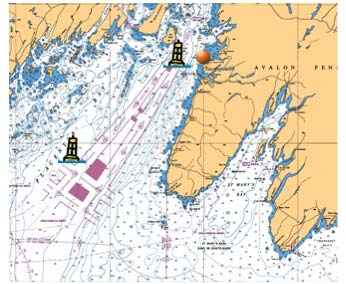
\includegraphics[width=0.5\linewidth]{figs/f4.jpg}
       \caption{The locations of two buoys (the two towers) and a single
    radar site (orange button). The bottom left buoy is at at the mouth
    of Placentia Bay, and the top right buoy is at the Pilot Boarding
    Station at the south end of Red Island.}
  \end{figure}
\end{frame}

\begin{frame}
  \begin{figure}[htbp]
  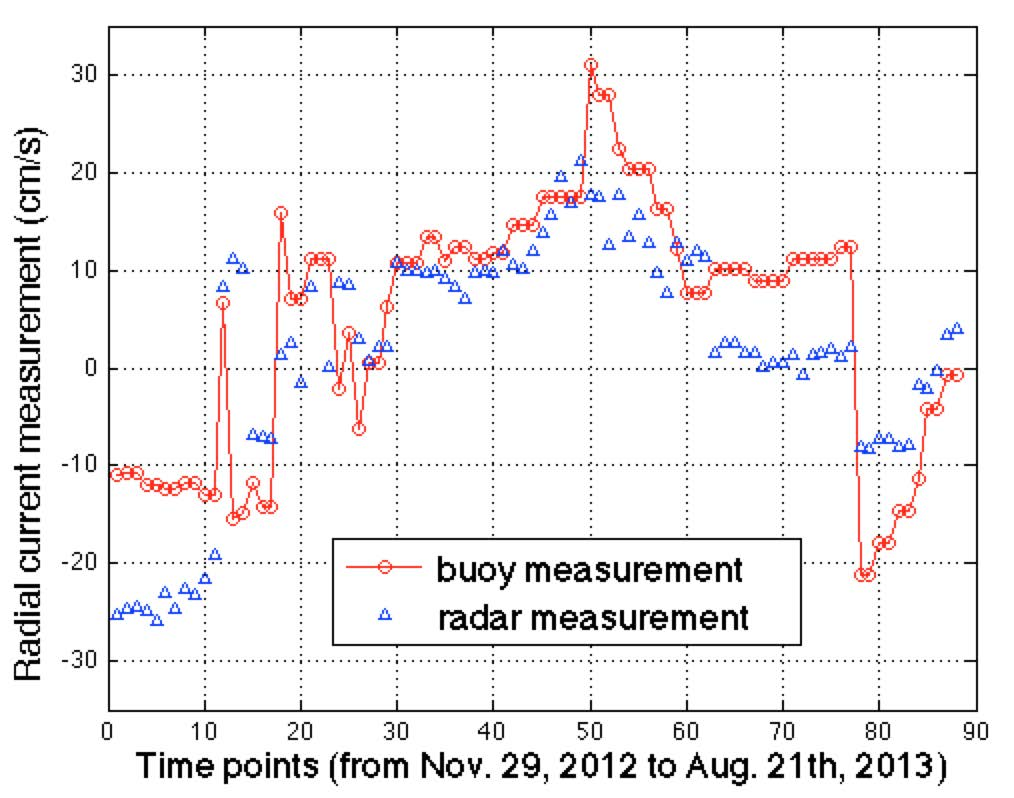
\includegraphics[width=0.5\linewidth]{figs/a.jpg}
       \caption{MUSIC, p=3, centroid, cor=0.77,
       rms=8.84 cm/s}
      \end{figure}
\end{frame}
\begin{frame}
  \begin{figure}[htbp]
      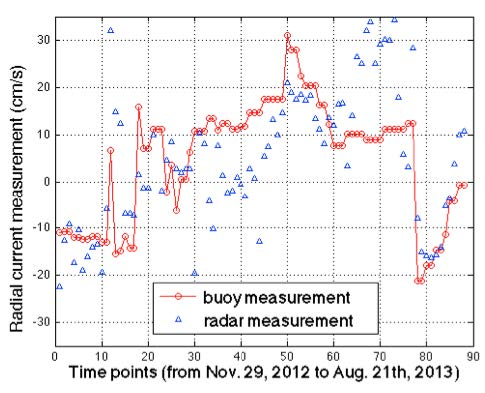
\includegraphics[width=0.5\linewidth]{figs/b.jpg}
       \caption{AR, p=14, centroid, cor=0.61,
       rms=12.17 cm/s}
  \end{figure}
\end{frame}

\begin{frame}
  \begin{figure}[htbp]
      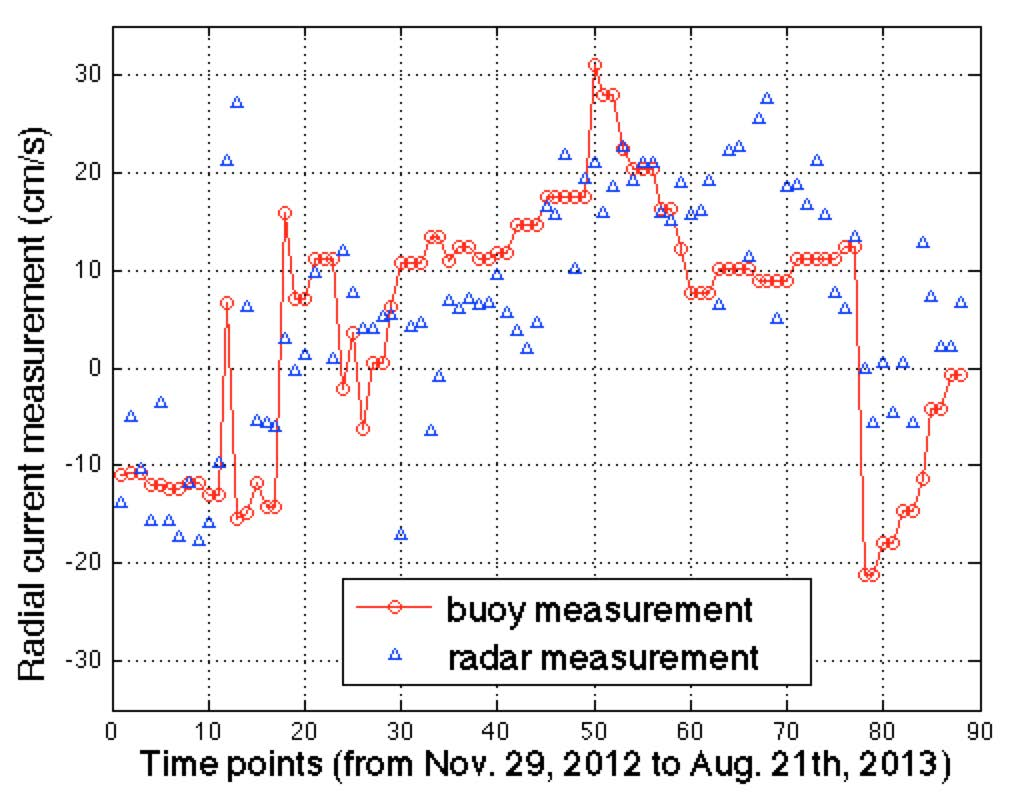
\includegraphics[width=0.5\linewidth]{figs/c.jpg}
       \caption{WELCH, centroid, cor=0.63,
       rms=10.69 cm/s}
  \end{figure}
\end{frame}

\begin{frame}
  \begin{figure}[htbp]
      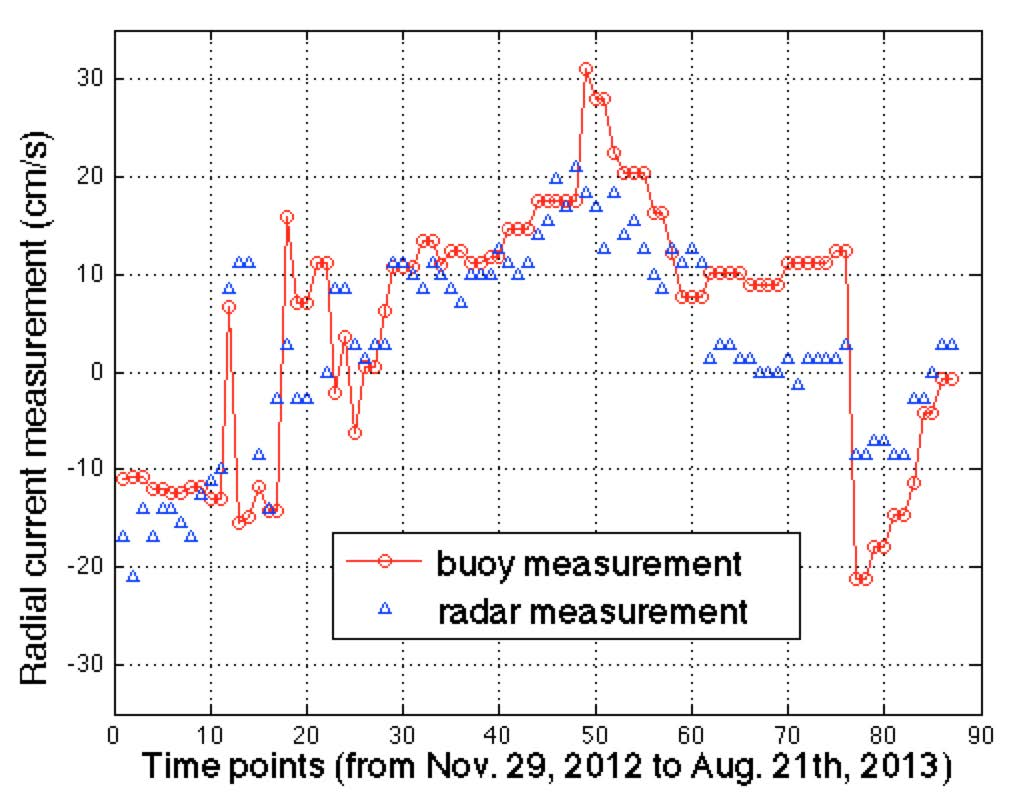
\includegraphics[width=0.5\linewidth]{figs/d.jpg}
       \caption{MUSIC, p=3, SPS, cor=0.79, rms=8.03
       cm/s}
  \end{figure}
\end{frame}

\begin{frame}
  \begin{figure}[htbp]
      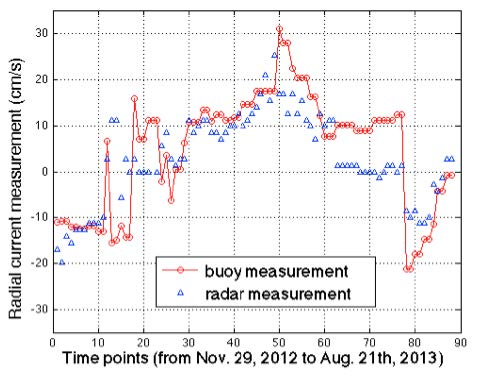
\includegraphics[width=0.5\linewidth]{figs/e.jpg}
       \caption{AR, p=14, SPS, cor=0.77, rms=8.27
       cm/s}
  \end{figure}
\end{frame}

\begin{frame}
  \begin{figure}[htbp]
      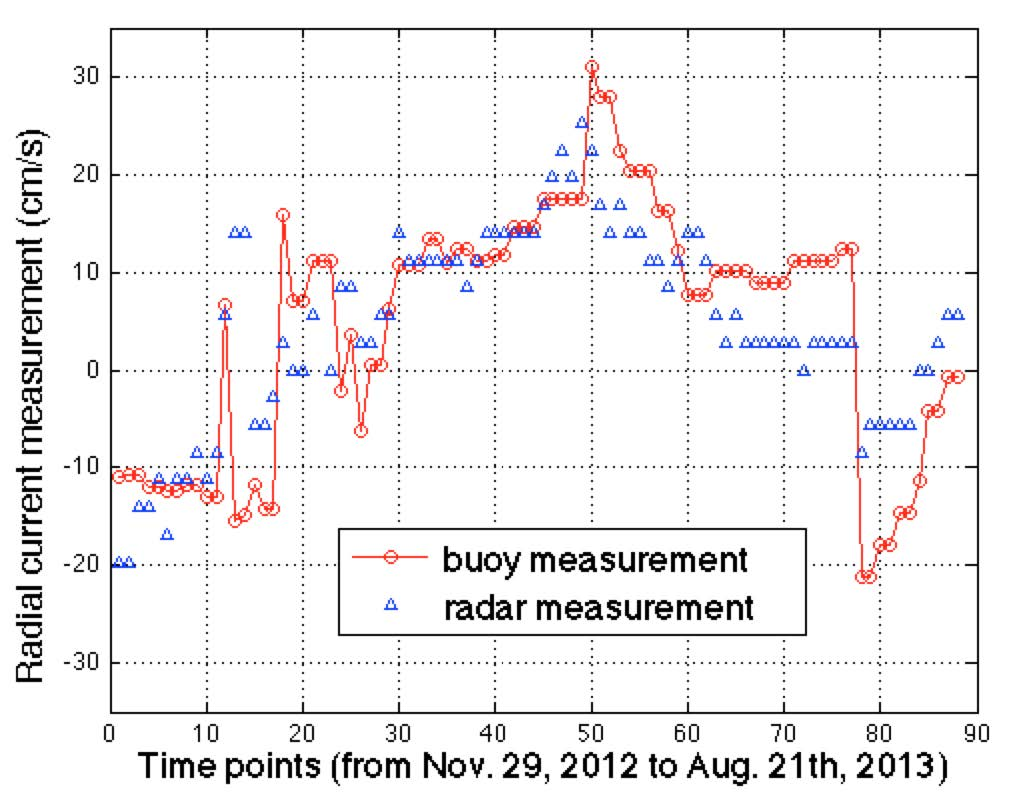
\includegraphics[width=0.5\linewidth]{figs/f.jpg}
       \caption{WELCH, SPS, cor=0.77, rms=8.16 cm/s}
  \end{figure}
\end{frame}

\begin{frame}
  \begin{figure}[htbp]
      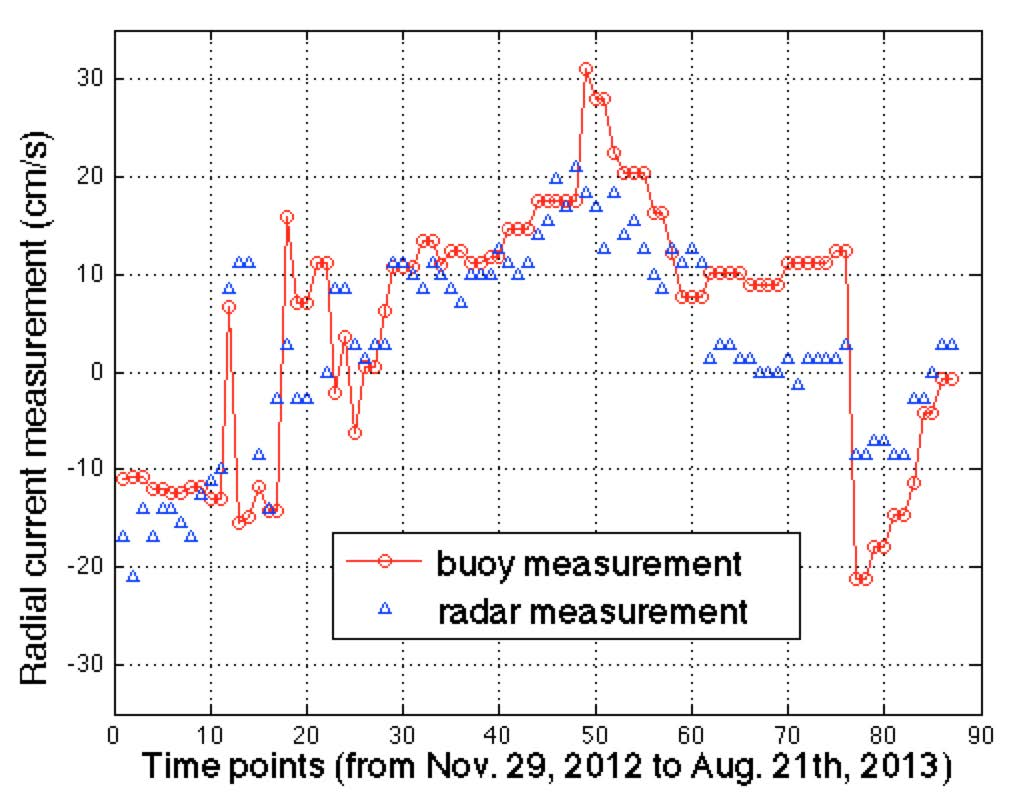
\includegraphics[width=0.5\linewidth]{figs/g.jpg}
       \caption{MUSIC, p=3, GA/SPS, cor=0.79,
       rms=8.03 cm/s}
  \end{figure}
\end{frame}

\begin{frame}
  \begin{figure}[htbp]
      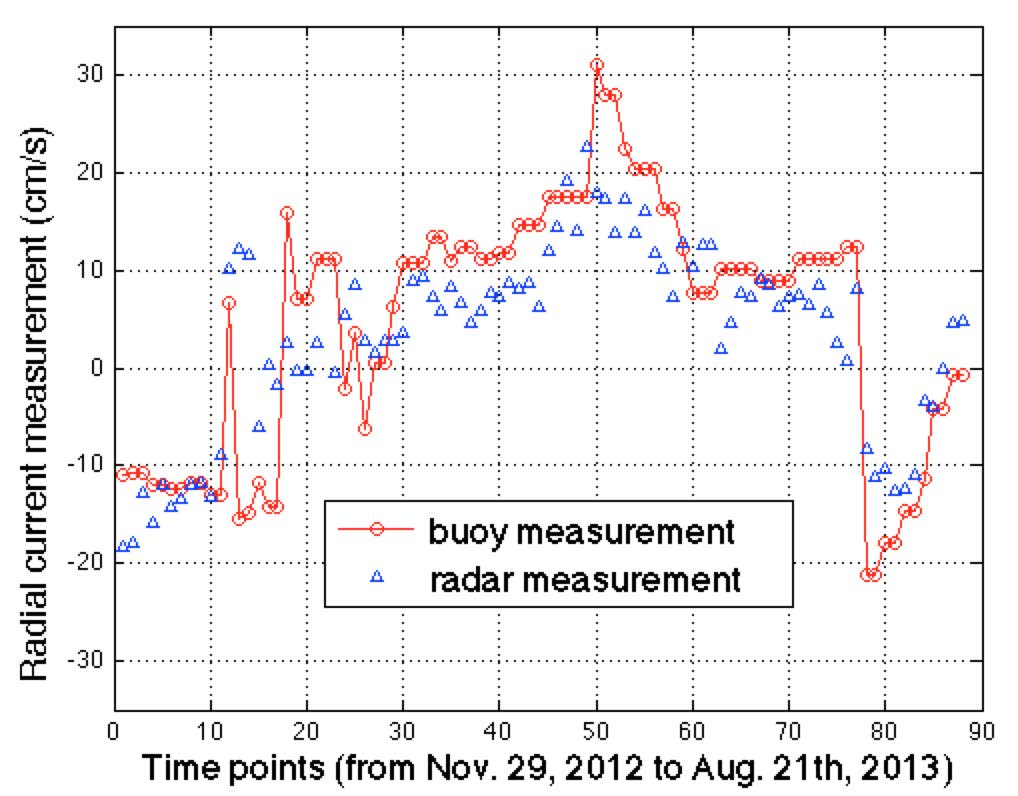
\includegraphics[width=0.5\linewidth]{figs/h.jpg}
       \caption{AR, p=14, GA, cor=0.81, rms=7.58
       cm/s}
  \end{figure}
\end{frame}
\begin{frame}
  \begin{figure}[htbp]
      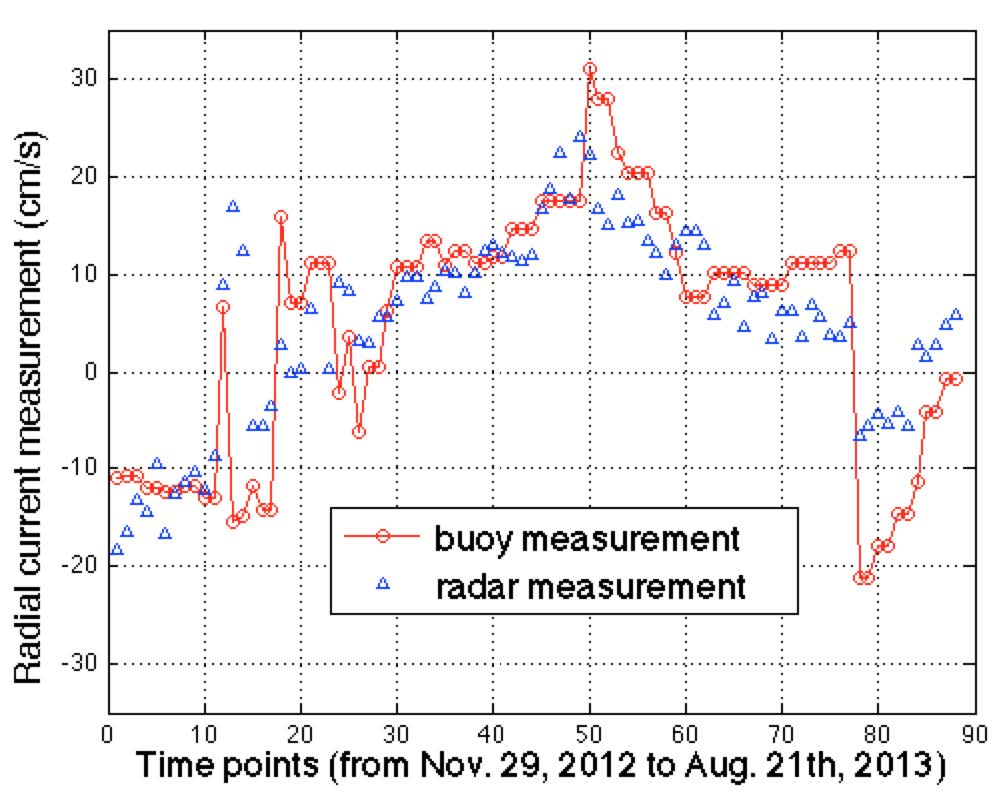
\includegraphics[width=0.5\linewidth]{figs/i.jpg}
       \caption{WELCH, GA, cor=0.79, rms=7.92 cm/s}
  \end{figure}
\end{frame}
\begin{frame}{}
  \begin{table}
    \begin{tabular}{|p{1.5cm}cc|p{1.5cm}cc|p{1.5cm}cc|}
      \hline
      Method&cor&rms&Method&cor&rms&Method&cor&rms\\
      \hline
      \hline
      MUSIC, centroid&0.77&8.84& AR, centroid&0.61&12.17&Welch, centroid&0.63&10.69\\
      \hline
      MUSIC, SPS& 0.79&8.03&AR, SPS&0.77&8.27&Welch, SPS&0.77&8.16\\ \hline
      MUSIC, GA/SPS&0.79&8.03&AR, GA&0.81&7.58&Welch, GA &0.79& 7.92\\
      \hline
    \end{tabular}
  \end{table}
\end{frame}

\section{Conclusion}
\begin{frame}{Outline}
  \transfade%淡入淡出效果
  \tableofcontents[sectionstyle=show/shaded,subsectionstyle=show/shaded] %这几个参数我也不知道该如何准确地解释,反正它们最终的效果是突出显示当前章节,而其它章节都进行了淡化处理
  %\addtocounter{framenumber}{-1}  %目录页不计算页码
\end{frame}
\begin{frame}{5. Conclusion}
  \begin{itemize}
    \item In this paper, the conventional periodogram method (i.e. Welch) and high-resolation spectral estimation methods (i.e. AR and MUSIC) were investigated in conjunction with two Bragg identification methods (i.e. the centroid and the SPS methods). \newline
    \item The SPS method exhibited significant imporvement over the centroid method for all three SE techniques.
  \end{itemize}
\end{frame}
\begin{frame}{5. Conclusion}
  \begin{itemize}
    \item A weigthed sum of the radar currents estimated by the SPS and the centroid methods is found to reduce the rms difference from the buoy currents.\newline
    \item A genetic algorithm has been successfully implemented to find the global solution for the optimal weighting ratio. \newline
    \item This ratio is found to be 85\%, 75\%and 100\% for Welch, AR, and MUSIC methods.
  \end{itemize}
\end{frame}


\section{Reference}

\begin{frame}{Reference}
  \bibliographystyle{IEEEtran}
  \bibliography{reference.bib}
\end{frame}

\begin{frame}

\begin{center}
	\huge \textbf{Thanks Listening\\ \& Best Regards !}
\end{center}
	
\end{frame}
\end{document}
